\chapter{Rete e coordinamento della mesh}
\label{chap:rete}

\section{Politiche di rete e confini di reachability}

Le trust zones della \autoref{fig:trust-zones} descrivono chi può contattare chi. I confini di reachability
che ne derivano sono resi effettivi da una politica di rete che Network-Manager pubblica su Headscale.

Ogni nodo della rete mesh, sia esso un servizio o il dispositivo di un utente, porta una o più etichette
chiamate tag. Le regole di raggiungibilità sono scritte sui tag anziché su indirizzi IP, in modo da 
sopravvivere al cambiamento di indirizzo di un servizio, dovuto ad esempio al suo riavvio su un nodo diverso.

Network-Manager raccoglie tutte le regole in un unico documento e lo consegna a Headscale una sola volta,
all'avvio \cite{ramusb-code-acl-policy}. 

Headscale a sua volta lo traduce in un filtro dei pacchetti: a ogni nodo che entra nella rete comunica solo i
peer che le regole gli permettono di contattare, insieme ai propri aggiornamenti successivi.
In questo modo, un servizio che da regolamento non deve contattarne un'altro, non è nemmeno in grado di 
vederlo nella rete.

Le regole, inoltre, nominano soltanto chi apre la connessione, quindi le risposte viaggiano senza una regola 
nel verso opposto. In questo modo, ad esempio, Security-Switch può contattare Database-Vault, e quest'ultimo 
può rispondere alla richiesta, ma non è in grado di avviare una comunicazione con lui. 

\section{Ciclo di vita dei grant di accesso}

Le due regole che riguardano l'utente sono riportate nel \autoref{lst:acl-utente}. Il tag 
\texttt{TagStorageAccess} è temporaneo e viene assegnato al login; \texttt{TagMeshMember} è permanente e 
viene assegnato quando il dispositivo entra nella rete.

\Needspace{12\baselineskip}
\begin{lstlisting}[caption={Le due regole che delimitano le zone dell'utente, da \texttt{policy.go}
\cite{ramusb-code-acl-policy}, con commenti aggiunti.}, label={lst:acl-utente}]
{ // solo un utente autenticato, e Database-Vault, raggiungono Storage-Service
    Action: "accept",
    Src:    []string{TagStorageAccess, TagDatabaseVault},
    Dst:    []string{dstAny(TagStorageService)},
},
{ // ogni utente registrato raggiunge Entry-Hub
    Action: "accept",
    Src:    []string{TagMeshMember},
    Dst:    []string{dstAny(TagEntryHub)},
},
\end{lstlisting}

Alla registrazione, Network-Manager crea per il nuovo utente un'identità su Headscale e una pre-auth key,
cioè una credenziale monouso con cui il dispositivo si presenta al coordinatore per entrare nella rete
\cite{ramusb-code-mesh-user}. La chiave vale quindici minuti, e risale la catena dei servizi fino
all'utente dentro la risposta alla registrazione.

La chiave nasce già associata al tag di sola appartenenza. Il dispositivo che la usa entra quindi nella
rete e ottiene la raggiungibilità verso l'interfaccia di rete privata di Entry-Hub.

Al login Network-Manager cerca il nodo dell'utente e gli aggiunge il secondo tag, poi annota la scadenza a 
dodici ore da quel momento \cite{ramusb-code-grant}.

La ricerca del nodo dell'utente richiede però che Network-Manager tenga un piccolo database SQLite
contenente l'identificativo numerico della pre-auth key legata all'hash dell'email dell'utente, con lo
schema riportato nel \autoref{lst:meshusers-schema}.

\Needspace{8\baselineskip}
\begin{lstlisting}[language=sql, caption={Schema della tabella di corrispondenza email-pre-auth-key, da
\texttt{meshusers.go} \cite{ramusb-code-meshusers-schema}.}, label={lst:meshusers-schema}]
CREATE TABLE IF NOT EXISTS mesh_users (
	email_hash       TEXT PRIMARY KEY,
	pre_auth_key_id  INTEGER NOT NULL
);
\end{lstlisting}

Anche le scadenze dei tag sono persistite sul database, per evitare che un riavvio del servizio trasformi 
un permesso di dodici ore in un permesso perpetuo. Lo schema della tabella che le contiene è riportato nel
\autoref{lst:grants-schema}.

\Needspace{10\baselineskip}
\begin{lstlisting}[language=sql, caption={Schema della tabella dei grant di accesso, da \texttt{store.go}
\cite{ramusb-code-grants-schema}.}, label={lst:grants-schema}]
CREATE TABLE IF NOT EXISTS grants (
	email_hash TEXT PRIMARY KEY,
	node_id    INTEGER NOT NULL,
	tag        TEXT NOT NULL,
	expires_at INTEGER NOT NULL
);
\end{lstlisting}

Un processo periodico, ogni cinque minuti, cerca le scadenze passate e revoca i grant scaduti
\cite{ramusb-code-sweep}. La riga viene cancellata dal database prima di chiamare Headscale per togliere 
il tag, e la cancellazione è condizionata alla scadenza esatta appena letta.
Se nel frattempo un login ha rinnovato il grant, la scadenza in tabella non coincide più, la cancellazione
non tocca nessuna riga, e lo sweep si ferma senza contattare Headscale. 
Chiamare prima Headscale e cancellare poi avrebbe invece rischiato di cancellare anche la riga
appena riscritta dal login concorrente, togliendo all'utente un permesso appena concesso.

La \autoref{fig:acl-grant} riassume gli stati che il nodo di un utente attraversa.

\begin{figure}[H]
    \centering
    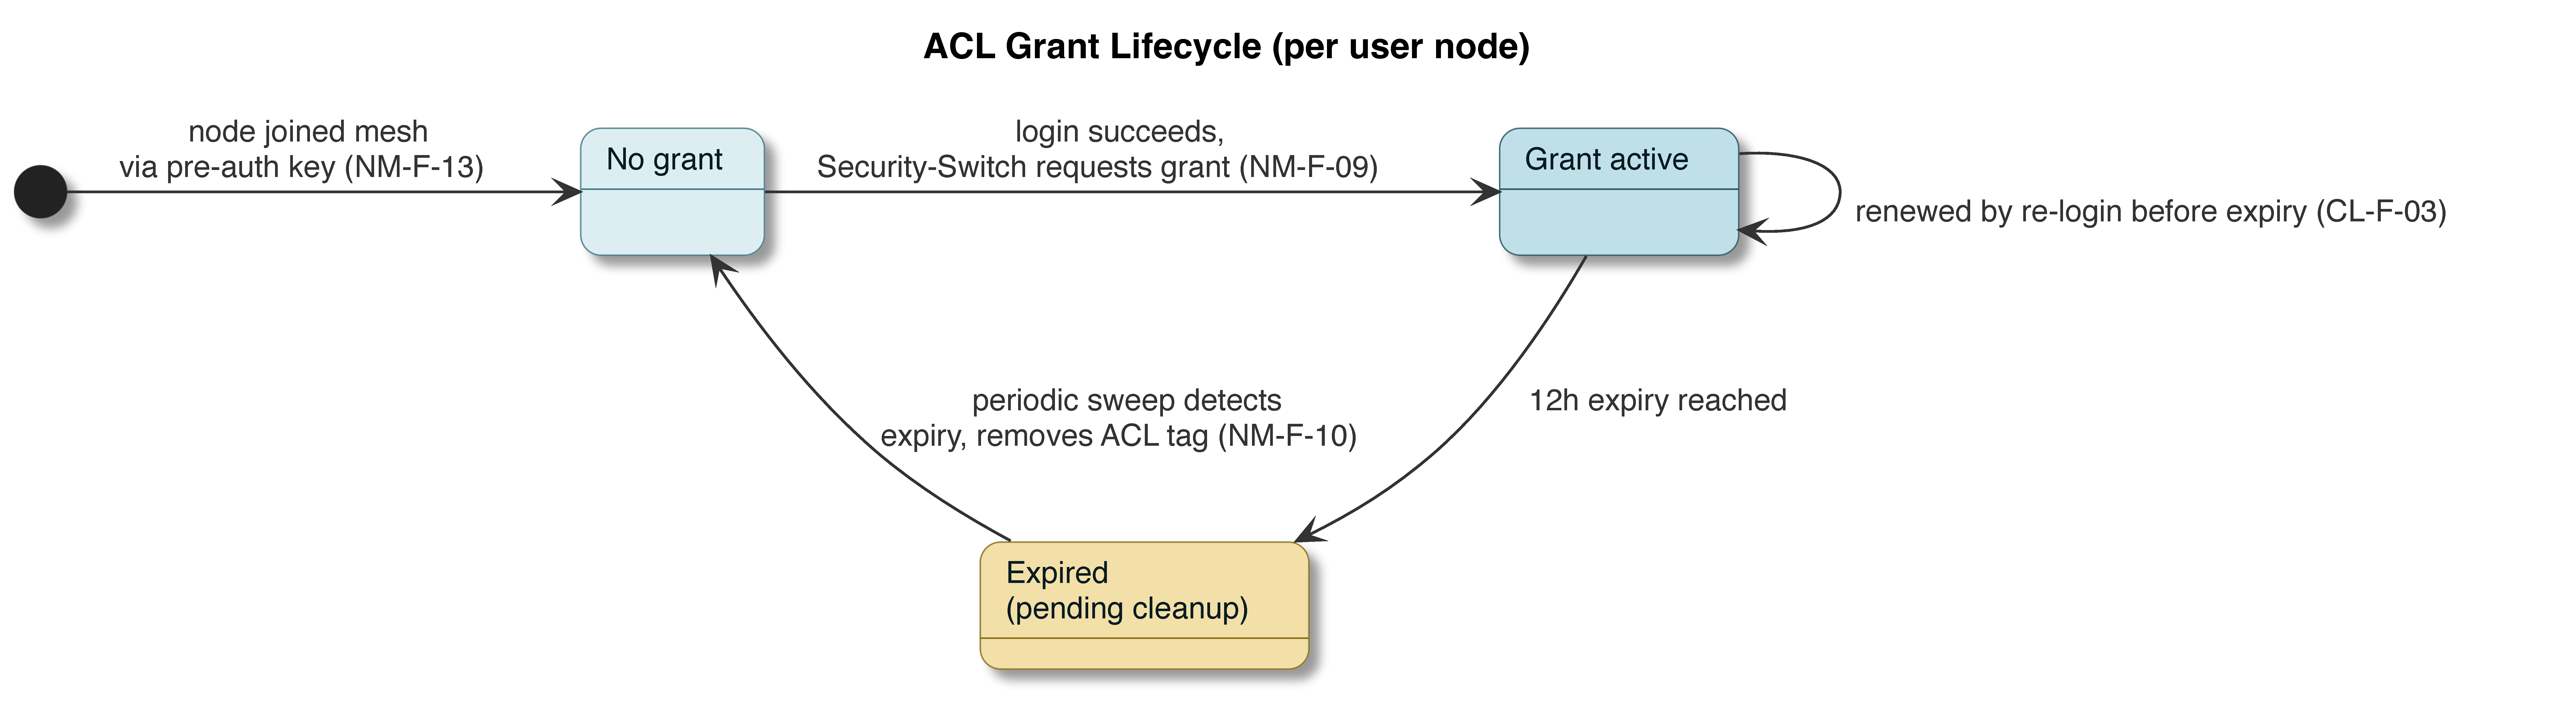
\includegraphics[width=\textwidth]{figures/10-operations-state-acl-grant.pdf}
    \caption{Ciclo di vita del permesso di accesso associato al nodo di un utente.}
    \label{fig:acl-grant}
\end{figure}


\section{Il paradosso del coordinatore: Headscale come servizio a sé}
\label{sec:paradosso-coordinatore}

La documentazione di Headscale dichiara che non è consigliato eseguire Headscale su una macchina che 
appartiene alla rete coordinata, perché può creare problemi alla risoluzione dei nomi tramite MagicDNS 
\cite{headscale-faq}. 

Il coordinatore deve perciò restare estraneo alla rete che coordina, e da qui discendono tre conseguenze.

La prima è che non può condividere una macchina virtuale o un container con nessun altro componente, 
perché tutti gli altri sono membri della mesh.

La seconda è che il traffico con cui Network-Manager crea le chiavi e assegna i tag non può essere
protetto dalla collocazione in rete, come invece accade per ogni altra chiamata interna. È l'unica
chiamata tra componenti del sistema che attraversa la rete pubblica, e l'unica la cui protezione dipende
interamente da mTLS.

La terza è che il coordinatore deve essere raggiungibile pubblicamente, perché un dispositivo che non è
ancora entrato nella rete deve poterlo contattare la prima volta per poter entrare nella rete.

Headscale ha però una limitazione rilevante per RAM-USB: non offre alcun modo di separare il protocollo di 
coordinamento, che deve essere raggiunto da tutti, dall'API amministrativa, che deve essere raggiunta solo da
Network-Manager. 
La separazione è stata affidata a un reverse proxy, che distingue le due superfici in base al percorso
della richiesta \cite{ramusb-code-headscale-proxy}. Le richieste di coordinamento passano senza alcun controllo,
mentre quelle amministrative sono accettate solo se accompagnate da un certificato emesso dalla 
Certificate-Authority privata, a cui si aggiunge anche una chiave API che Headscale richiede per conto 
proprio. Il traffico amministrativo è difeso da due credenziali indipendenti perché è una delle superfici 
più sensibili.

Il certificato presentato dal proxy è invece emesso da una CA pubblica, per la stessa ragione per cui lo
è quello di Entry-Hub. 

\section{CG-NAT e la necessità di un endpoint pubblico dedicato}

Visto che gli indirizzi IPv4 sono ormai terminati, gli Internet Service Providers assegnano ai router 
domestici dei clienti un IPv4 condiviso tra più clienti nel range \texttt{100.64.0.0/10} 
rendendo impossibile ai clienti esporre un proprio server su internet. Questo tipo di natting prende il nome
di Carrier-Grade NAT \cite{rfc6598}.
Visto che RAM-USB è progettato per essere hostato anche da utenti consumer, che potrebbero quindi non possedere
un IPv4 pubblico o un IPv6, Headscale ed Entry-Hub risiedono su un Virtual Private Server, separato dal 
resto del sistema. Il \autoref{chap:deployment} descrive la collocazione effettiva di ciascun componente.
